\chapter{Do-Calculus}\label{chap-do-calc}


The Do-calculus and associated ideas were
invented by
Judea Pearl and collaborators.
This chapter is heavily
based on Judea Pearl's
books. (See \ref{ch-nav-pearl}).


$\rvX.=\rvV. \cup \rvH.$,
$\rvV. \cap \rvH.=\emptyset$.
$\rvV.$= visible, observed.
$\rvH.$= hidden, uobserved.
Hidden nodes will 
be indicated 
either
by
enclosing
them their random variable
in a box (as
if it were a black box) or
by making
the arrows
coming
out of them
dashed.

\beq
\xymatrix{
&*+[F]{\rvc}\ar[dl]\ar[dr]
\\
\rvx\ar[rr]&&\rvy
}
\;\;\;
\xymatrix{
\rvx\ar@{-->}@{<-->}@/^2pc/[rr]
\ar[rr]&&\rvy
}
\;\;\;
\xymatrix{
&\rvc\ar@{-->}[dl]\ar@{-->}[dr]
\\
\rvx\ar[rr]&&\rvy
}
\eeq

\begin{figure}[h!]
\centering
\includegraphics[width=4in]
{do/do-rho-lam.png}
\caption{
The operator $\rho_\rvx$
converts node $\rvx$
into a root node $\rho \rvx$.
The operator $\lam_\rvx$
converts node $\rvx$
into a leaf node $\lam\rvx$.
} 
\label{fig-do-rho-lam}
\end{figure}

\beq
\rho_{\rva.}G =
\prod_j \rho_{\rva_j}G
\;,\;\;\;\;
\lam_{\rva.}G =
\prod_j \lam_{\rva_j}G
\eeq

\beq
P(X.-a.|\rho\rva.=a.)
=
\caln(!(X.-a.))
\prod_{j:\rvX_j\notin \rva.}
P(X_j|pa(X_j))
\eeq

$\rvb.\subset \rvX.-\rva.$
\beq
P(b.|\rho\rva. =a.)=
\sum_{X.-a.-b.}
P(X.-a.|\rho\rva.=a.)
\eeq

$\rvr.\subset \rvX.-\rva.-\rvb.$
\beq
P(b.|\rho \rva.=a., r.)=
\frac{P(b., r.|\rho\rva.=a.)}
{P(r.|\rho\rva.=a.)}
\eeq



Usually
$P(b.|\rho \rva.=a., s.)$
is denoted by
$P(b.|do(\rva.=a.), s.)$.



$P(b.|\rho \rva.=a., s.)$
is said to be {\bf identifiable}
if it can be
expressed as a product of
conditional prob distributions
that only
depend on observed 
variables and that
have no $do()$
conditions in them.

For $\rvx, rvy\in \bool$,
``causal effect difference¨ ,
or `average causal effect¨ (ACE)
\beq
ACE=
P(y=1|\rho \rvx=1)-
P(y=1|\rho \rvx=0)
\eeq
Risk Difference
\beq
RD=
P(y=1|\rvx=1)-
P(y=1|\rvx=0)
\eeq


\section*{3 Rules of do-calculus}

If $(\rvb.\perp \rva.|\rvr., \rvs.)$
in $G$, then $P(b.|a., r., s.)=P(b.|r., s.)$

\begin{color}{red}
\begin{itemize}
\item {\bf Rule 1:} 
Insertion or deletion of
 observations ($\rva.=a. \leftrightarrow 1$ )

\ruleone

\item {\bf Rule 2:} Action or 
observation exchange 
($\rho \rva.=a. \leftrightarrow \rva.=a.$)

\ruletwo

\item {\bf Rule 3:} Insertion and
 deletion of actions
($\rho \rva.=a. \leftrightarrow 1$)

\rulethree


\end{itemize}
\end{color}


\section*{Backdoor Adjustment}
Back and front
door {\bf adjustment formulas}.
Adjust a variable , average
over it, control it.

See Chapter \ref{chap-bdoor}
for examples of the use of the 
backdoor adjustment formula.
In this section,
we are mainly
concerned with
proving that
formula
using do-calculus.



\bdoordef
\begin{claim} Backdoor Adjustment

\bdoorclaim
\end{claim}
\proof
\beq
\xymatrix{
{\rvz}\ar[d]\ar[rd]
\\
\rvx\ar[r]&\rvy
}
\eeq
\beq
\begin{array}{lllll}
&&\color{red}
P(y|\rho\rvx=x)=
\\
&=&
\color{red}
\sum_m 
P(y|\rho\rvx=x, z)
P(z|\rho\rvx=x) 
\\
&&\text{by Probability Axioms}
\\
&=&\color{red}
\sum_ 
P(y|x, z)
P(z|\rho\rvx=x)
\\
&&P(y|\rho \rvx=x, z)\rarrow
P(y|x, z)
\\
&& \text{ by Rule 2: \ruletwo}
\\
&&
\rvy\perp \rvx|\rvz
\text{ in }\lam_\rvx G
\;\;\;\;
\xymatrix{
{\rvz}\ar[d]\ar[rd]
\\
\rvx&\rvy
}
\\
&=&\color{red}
\sum_z 
P(y|x, z)
P(z)
\\
&&P(z|\rho \rvx=x)\rarrow
P(z)
\\
&& \text{ by Rule 3: \rulethree}
\\
&&
\rvz\perp \rvx
\text{ in }\rho_\rvx G
\;\;\;\;
\xymatrix{
{\rvz}\ar[rd]
\\
\rvx\ar[r]&\rvy
}
\end{array}
\eeq
\qed

\beqa
P(y.|\rho \rvx. =x.)
&=&
\sum_{z.}P(y.|x., z.)P(z.)
\\
&=&
\sum_{z.}\frac{P(y.,x., z.)}
{P(x.|z.)}
\eeqa
$P(x.|z.)$ called propensity
score, can be approximated.

\section*{Front Door Adjustment}
See Chapter \ref{chap-fdoor}
for examples of the use of the 
backdoor adjustment formula.
In this section,
we are mainly
concerned with
proving that
formula
using do-calculus.

\fdoordef

\begin{claim} Front-Door Adjustment

\fdoorclaim

\end{claim}
\proof
$\rvc$ confounder, hidden

\beq
\xymatrix{
&*+[F]{\rvc}\ar[ld]\ar[rd]
\\
\rvx\ar[r]&\rvm\ar[r]&\rvy
}
\eeq

\beq
\begin{array}{lllll}
&&\color{red}
Pcc(y|\rho\rvx=x)=
\\
&=&
\color{red}
\sum_m 
P(y|\rho\rvx=x, m)
P(m|\rho\rvx=x) 
\\
&&\text{by Probability Axioms}
\\
&=&\color{red}
\sum_m 
P(y|\rho\rvx=x, \rho\rvm=m)
P(m|\rho\rvx=x)
\\
&&P(y|\rho\rvx=x, m)\rarrow
P(y|\rho\rvx=x, \rho m=m)
\\
&& \text{ by Rule 2: \ruletwo}
\\
&&
\rvy\perp \rvm|\rvx
\text{ in }\lam_\rvm\rho_\rvx G
\xymatrix{
&*+[F]{\rvc}\ar[rd]
\\
\rvx\ar[r]&\rvm&\rvy
}
\\
&=&\color{red}
\sum_m 
P(y|\rho\rvx=x, \rho\rvm=m)
P(m| x)
\\
&&
P(m|\rho\rvx=x)\rarrow P(m|x)
\\
&&\text{by Rule 2: \ruletwo}
\\
&&
\rvm\perp\rvx
\text{ in }
\lam_\rvx G
\xymatrix{
&*+[F]{\rvc}\ar[ld]\ar[rd]
\\
\rvx&\rvm\ar[r]&\rvy
}
\\
&=&\color{red}
\sum_m 
P(y|\rho\rvm=m)
P(m|x)
\\
&&
P(y|\rho\rvx=x, \rho\rvm=m)
\rarrow
P(y|\rho\rvm=m)
\\
&&\text{by Rule 3: \rulethree}
\\
&&
\rvy\perp\rvx|\rvm
\text{ in }
\rho_\rvx\rho_\rvm G
\xymatrix{
&*+[F]{\rvc}\ar[rd]
\\
\rvx&\rvm\ar[r]&\rvy
}
\\
&=&\color{red}
\sum_{x'}
\sum_m 
P(y|\rho\rvm=m, x')
P(x'|\rho\rvm=m)
P(m|x)
\\
&&\text{by Probability Axioms}
\\
&=&\color{red}
\sum_{x'}
\sum_m 
P(y|m, x')
P(x'|\rho\rvm=m)
P(m|x)
\\
&&
P(y|\rho\rvm=m, x')
\rarrow
P(y|m, x')
\\
&& \text{by Rule 2: \ruletwo}
\\
&&
\rvy\perp\rvm|\rvx
\text{ in }
\lam_\rvm G
\xymatrix{
&*+[F]{\rvc}\ar[rd]\ar[ld]
\\
\rvx\ar[r]& \rvm&\rvy
}
\\
&=&\color{red}
\sum_{x'}
\sum_m 
P(y|m, x')
P(x')
P(m|x)
\\
&&
P(x'|\rho\rvm=m)
\rarrow
P(x')
\\
&&\text{by Rule 3: \rulethree}
\\
&&
\rvx\perp\rvm
\text{ in }
\rho_\rvm G
\xymatrix{
&*+[F]{\rvc}\ar[rd]\ar[ld]
\\
\rvx&\rvm\ar[r]&\rvy
}
\end{array}
\eeq
\qed


